\documentclass[11pt,letterpaper]{article}
\usepackage{fullpage}
\usepackage[pdftex]{graphicx}
\usepackage{amsfonts,eucal,amsbsy,amsopn,amsmath}
\usepackage{url}
\usepackage[sort&compress]{natbib}
\usepackage{natbibspacing}
\usepackage{latexsym}
\usepackage{wasysym} 
\usepackage{rotating}
\usepackage{verbatim}
\usepackage{fancyhdr}
\DeclareMathOperator*{\argmax}{argmax}
\DeclareMathOperator*{\argmin}{argmin}
\usepackage{sectsty}
\usepackage[dvipsnames,usenames]{color}
\usepackage{multicol}
\definecolor{orange}{rgb}{1,0.5,0}
\usepackage{multirow}
\usepackage{algorithm}
\usepackage{algorithmic,latexsym}
\usepackage{sidecap}
\usepackage{caption}
\renewcommand{\captionfont}{\small}
\setlength{\oddsidemargin}{-0.04cm}
\setlength{\textwidth}{16.59cm}
\setlength{\topmargin}{-0.04cm}
\setlength{\headheight}{0in}
\setlength{\headsep}{0in}
\setlength{\textheight}{22.94cm}
\allsectionsfont{\normalsize}
\newcommand{\ignore}[1]{}
\newcommand{\thedate}{\today}
\newenvironment{enumeratesquish}{\begin{list}{\addtocounter{enumi}{1}\arabic{enumi}.}{\setlength{\itemsep}{-0.25em}\setlength{\leftmargin}{1em}\addtolength{\leftmargin}{\labelsep}}}{\end{list}}
\newenvironment{itemizesquish}{\begin{list}{\setcounter{enumi}{0}\labelitemi}{\setlength{\itemsep}{-0.25em}\setlength{\labelwidth}{0.5em}\setlength{\leftmargin}{\labelwidth}\addtolength{\leftmargin}{\labelsep}}}{\end{list}}

\bibpunct{(}{)}{;}{a}{,}{,}
\newcommand{\nascomment}[1]{\textcolor{blue}{\textbf{[#1 --NAS]}}}


\pagestyle{fancy}
\lhead{}
\chead{}
\rhead{}
\lfoot{}
\cfoot{\thepage~of \pageref{lastpage}}
\rfoot{}
\renewcommand{\headrulewidth}{0pt}
\renewcommand{\footrulewidth}{0pt}


\title{11-712:  NLP Lab Report\\
\textbf{Dependency Parsing for Weibo:\\
A Dependency Arc Inference Approach using Efficient First-Order Probabilistic Logic Programming}}
\author{William Wang\\
ww@cmu.edu}
%\data{January 17, 2014}
\date{\today}

\begin{document}
\maketitle
\begin{abstract}
Dependency parsing is a core task in NLP, and it is a widely used by many applications such as information extraction,
question answering, and machine translation. In general, the resources for Chinese dependency parsing are less accessible than English, and publicly available Chinese dependency parsers are still very limited. In this project, the goal is to build a Chinese dependency parser for Weibo --- China's equivalent of Twitter. 
To do this, we formulate the dependeny parsing problem as many small and parallelizable structure prediction tasks:
for each task, we use a locally groundable probabilistic first-order logic to infer the dependency arc of a token in the sentence.
In experiments, we show that the proposed model outperforms an off-the-shelf Stanford Chinese parser,
and that leveraging lexical, syntactic, and distributional cues help improving the performance.
In addition to this, we provide a publicly available GFL/FUDG-annotated Weibo treebank.

\end{abstract}

\section{Basic Information about Chinese Dependency Parsing}
\label{sec:info}
Chinese dependency parsing has attracted many interests in the past decade.
\cite{bikel2000two} and \citet{Chiang:2002} are among the first to use Penn Chinese Tree Bank for dependency parsing,
where they adapted~\cite{xia1999extracting}'s head rules.
A few years later, the CoNLL shared task opened a track for multilingual dependency parsing,
which also included Chinese~\citep{buchholz2006conll,nilsson2007conll}.
These shared tasks soon popularized Chinese dependency parsing by making datasets available,
and there has been growing amount of literature since then~\citep{zhang2008tale,nivre2007maltparser,sagae2007dependency,
che2010ltp,carreras2007experiments,duan2007probabilistic}.
In this work, we aim at building a new publicly available Chinese dependency parsing tool, using 
a new parsing algorithm that leverages techniques from the field of statistical relational learning.

\section{Past Work on the Syntax of Chinese}
\cite{chao1968grammar} is among the first to study the syntax of Chinese. Unlike 
English, there has been long debate on the wordhood of Chinese~\citep{duanmu1998wordhood}.
Chao and others' work investigate the free and bound forms,
prosodic aspects~\citep{shen1990prosody}, semantics~\cite{li1972semantics,wu1999syntax}, and morphological aspects~\citep{tang1989studies,dai1992chinese,sproat2002corpus} to define the unit of word in Chinese.
In addition, he has also studied the complex compound constructions~\citep{zhou1999morphology,zhang2000extraction} in Chinese,
as well as the parts of speech such as nouns and verbs~\citep{krifka1995common}.
More recently, \cite{huang2009syntax} have studied
the lexical and functional categories,
argument structure, and the verb phrase in Chinese.
Moreover, they have discussed the more unique and challenging parts
of syntax in Chinese: the passives, the \emph{ba} construction,
and the topic \& relative constructions.
Interestingly, they have also shed light on some advanced Chinese linguistic issues 
that have not been well studied in the past: 
questions, nominal expressions, and anaphora.

Even though there has been many interesting linguistics papers on various aspects
of syntax in Chinese, the corresponding computational modeling work has been rather limited.
One of the most popular computational tasks in Chinese NLP is word segmentation~\citep{xue2003chinese,sproat2003first}.
where researchers have previously investigated sequencial models such as
hierarchial hidden Markov model~\citep{zhang2003hhmm}, maximum entropy Markov model~\citep{xue2003chinese}, and conditional random fields~\citep{zhao2006improved} for this task.
In addition to tokenization and segmentation, standard structure prediction tasks such as 
named entity recognition~\citep{xue2003chinese,wu2005chinese}, part-of-speech tagging~\citep{ng2004chinese,jiang2008cascaded}, and constituency parsing~\citep{wu1997stochastic,wang2006fast}
have also been studied in the language-specific setups.
As mentioned in Section~\ref{sec:info}, Chinese dependency parsing was first introduced
by \cite{bikel2000two}, and then became popular after the CoNLL multilingual shared tasks~\citep{buchholz2006conll,nilsson2007conll}.

In the past decade, there have been growing number of publicly availble Chinese language processing tools.
ICTCLAS\footnote{http://sewm.pku.edu.cn/QA/reference/ICTCLAS/FreeICTCLAS/English.html} is one of the most popular word segmentation tool in Chinese NLP. The Stanford Chinese NLP constituency parser~\citep{levy2003harder},
and the dependency parser~\citep{chang2009discriminative} also provide insights for many Chinese NLP applications.
More recently, more comphrehensive and Chinese-optimized toolkits were also made available~\citep{qiu2013fudannlp,che2010ltp}.
To the best of my knowledge, even though systems such as Malt parser~\citep{nivre2007maltparser} provides solutions 
to multilingual dependency parsing, but they are not optimized for Chinese, and the accuracy on Penn Chinese Treebank is
typically around 70\% and lower 80\%, which falls behind languages like English and German.

\section{Available Resources}
After some research and hands-on experiments on real data, I decided to use the open-source Stanford Word Segmenter\footnote{http://nlp.stanford.edu/software/segmenter.shtml} as the
segmentation tool. Comparing to other popular Chinese word segmenters, the Stanford segmenter
is well-maintained, and well-documented. The open-source Chinese lexicon I plan to use
is also attached in the distribution of Stanford Chinese Segmenter: the Penn Tree Bank lexicon
and the PKU lexicon. For the Chinese reference grammar, I am currently investigating the 
Stanford Dependencies\footnote{http://nlp.stanford.edu/software/stanford-dependencies.shtml},
but I am also open to other suggestions.

Both of my test datasets (TestA and TestB) are from a subset of Wang Ling's $\mu$topia Chinese microblog dataset\footnote{http://www.cs.cmu.edu/~lingwang/microtopia/}.
This dataset is very challenging for dependency parsing:
since pre-existing word segmentation and Chinese part-of-speech tagging tools 
are trained on standard Chinese news corpora, their perform poorly
on Weibo data. In addition to this, since Chinese is a pro-drop 
and topical language, finding the correct head verb for a long Weibo post 
could be very difficult.

\section{Survey of Phenomena in Chinese Dependency Parsing}
Like I mentioned in the previous section,
one notable difference between English and Chinese dependency parsing is the Chinese word segmentation issue,
while both English and Chinese parser may also suffer from the issue of part-of-speech tagging errors (due to train/test domain/genre mismatch).
However, despite these issues, there are still some interesting phenomena that mark the differences of the two languages:
\begin{itemize}
\item Function words are more frequently used in English than in Chinese.
For example, when examining Wang Ling's parallel English-Chinese for the total counts of the word ``the'',
there are 2,084 occurances in 2,003 sentences. Whereas in Chinese, there are only 52 occurances of the word 	``the'' 
out of the 2,003 sentences.
\item The other interesting thing is the position of the head. In English, it seems the head of the tree occurs more frequent
on the left-to-middle of the sentence, while the distribution of the head seems to be more complicated in Chinese.
This is also verified using the parallel Weibo data.
\item Another well-known issue in Chinese is that Chinese is a pro-drop language. 
This is extremely prominent in the short text. For example, in the Chinese Weibo data,
I have observed the sentence ``(If you) Want to eat Chicken, (you) Have to  bear the sounds of chickens.''.
\end{itemize}

\section{Initial Design}
I labeled Wang Ling's Weibo data with the help from many informant Lingpeng Kong.
We have set up an online annotation environment\footnote{http://www.ark.cs.cmu.edu:7788/annotate} ,
using the FUDG~\citep{schneider2013framework} and GFL annotation tool~\citep{chrissimplified} introduced by Nathan Schneider and Michael Mordowanec.
After discussing with my informant, we decide to start with the supervised learning approach.
This means that we need to have annotation additional datasets for training.
The training data has 2185 words, and the two test sets have 1020 and 1001 words respectively.

\begin{algorithm}[t] 
\small{
\caption{A Dependency Arc Inference Algorithm for Parsing Weibo} \label{alg1}
\begin{algorithmic}
\STATE Given: 
\STATE (1) a sentence with tokens $T_{i}$, where $i$ is the index, and $L$ is the length;
\STATE (2) a database $D$ of token relations from the corpus;
\STATE (3) first-order logic inference rule set $R$.
\STATE
\FOR{$i = 1 \to L$ tokens}
\STATE $\mathbb{S} \leftarrow ConstructSearchSpace(T_{i},R,D)$;
\STATE $\vec P_i \leftarrow InferParentUsingProPPR(T_{i},\mathbb{S})$;
\ENDFOR
\FOR{$i = 1 \to L$ tokens}
\STATE $Y_i = \arg\max \vec P_i$;
\ENDFOR
\end{algorithmic}}
\end{algorithm}

The main idea of the proposed algorithm
is that, instead of solving
the complex structure prediction problem as a whole,
we decompose the problem
into many parallelizable small local dependency arc inference task.
The algorithm is outlined in Algorithm\ref{alg1}.
For each of the tokens in a sentence,
we infer the parent token of this current token.
To do this, we make use of a recently proposed 
probabilistic first-order logic inference algorithm --- ProPPR~\citep{wangprogramming2013}.
ProPPR is an efficient graph inference framework
where the inference cost is independent of the size of the graph.
To construct the search space for ProPPR, 
we extract lexical and syntactic (part-of-speech) cues,
as well distributional information (e.g. adjacency or skip-$n$ grams)
to build the token-token relation database.
Then, we use simple inference rules to map 
the database to construct the search space.
In addition to this, we also need inference rules,
such as the following joint adjacency-skip-gram rules:

\begin{verbatim}
edge(V1,V2) :- 
               adjacent(V1,V2),hasword(V1,W1),
               hasword(V2,W2),keyword(W1,W2) #adjWord.

edge(V1,V2) :- 
               adjacent(V1,V2),haspos(V1,W1),
               haspos(V2,W2),keypos(W1,W2) #adjPos.

edge(V1,V2) :- 
               skipone(V1,V2),hasword(V1,W1),
               hasword(V2,W2),keysoword(W1,W2) #skiponeword.

edge(V1,V2) :- 
               skipone(V1,V2),haspos(V1,W1),
               haspos(V2,W2),keysopos(W1,W2) #skiponepos.

edge(V1,V2) :- 
               skiptwo(V1,V2),hasword(V1,W1),
               hasword(V2,W2),keystword(W1,W2) #skiptwoword.

edge(V1,V2) :- 
               skiptwo(V1,V2),haspos(V1,W1),
               haspos(V2,W2),keystpos(W1,W2) #skiptwopos.

edge(V1,V2) :- 
               skipthree(V1,V2),hasword(V1,W1),
               hasword(V2,W2),keysthword(W1,W2) #skipthword.

edge(V1,V2) :-
               skipthree(V1,V2),haspos(V1,W1),
               haspos(V2,W2),keysthpos(W1,W2) #skipthpos. 

keyword(W1,W2) :- # kw(W1,W2).
keypos(W1,W2) :- # kp(W1,W2).

keysoword(W1,W2) :- # ksow(W1,W2).
keysopos(W1,W2) :- # ksop(W1,W2).

keystword(W1,W2) :- # kstw(W1,W2).
keystpos(W1,W2) :- # kstp(W1,W2).

keysthword(W1,W2) :- # ksthw(W1,W2).
keysthpos(W1,W2) :- # ksthp(W1,W2).

\end{verbatim}
In the logic program above, we have a feature vector associated 
with each logic clause, and learning consists of tuning of the 
weights for each of the clause. Note that the last eight clauses
are templated logic clause, where it capture the co-occurrence
of two words/tags in a corpus.
We use~\cite{backstrom2011supervised}'s supervised variant
of personalized PageRank for learning, but with $tanh$ edge strength
function and a $L_2$-regularized log loss with parallel stochastic gradient descent.
After mapping the entities from the database to the logic program,
we can have the search graph in Fig.~\ref{fig:search}.
We refer to our prior work~\cite{wangprogramming2013} for the detailed inference algorithm.

\begin{figure*}[t]
\centerline{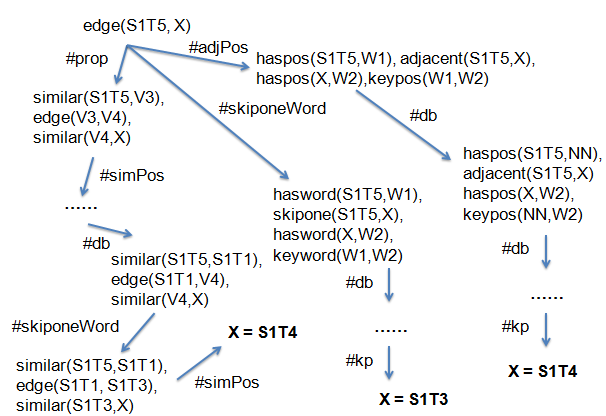
\includegraphics[scale=1]{search.png}}
\caption{A search graph generated from the initially design of the first-order logic inference clauses.}
\label{fig:search}
\end{figure*}

\section{System Analysis on Corpus A}
In the initial UAS result we obtain for corpus A,
we observe that if using the simple adjacency rule,
the UAS is 0.388. When using part-of-speech
information, we observe a result of 0.438.
When using the lexical information,
the UAS is 0.477. We also show 
some of the learned parameters in Fig.~\ref{fig:params}.

\begin{figure*}[t]
\centerline{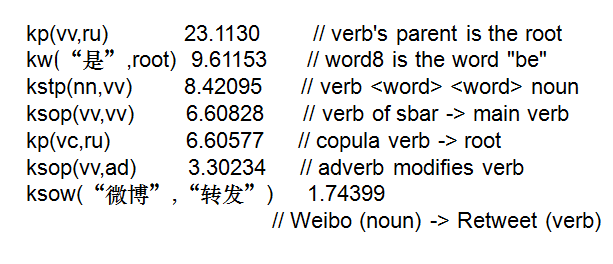
\includegraphics[scale=1]{learnedparameters.png}}
\caption{Some top-ranked parameters learned from the initially design of the first-order logic inference clauses.}
\label{fig:params}
\end{figure*}

\section{Lessons Learned and Revised Design}
From the learned parameter in Fig.~\ref{fig:params},
we can see that our model definitely captures some interesting
dependency structure from the data.
For example, we see that in the first parameter,
verb's parent is more likely to be the root.
Also, from the second rule, the copula verb ``be''
in Chinese is also likely to be pointed to the root.
In addition to that, we see that from the third parameter
that a noun is likely to be pointed to a verb if there are two words
in between them. 
To improve the performance of the parser,
we now consider the similarity clauses:

\begin{verbatim}
# similarity

edge(V1,V2) :- similar(V1,V3),edge(V3,V4),similar(V4,V2)  #prop.
similar(V1,V2) :- samesent(V1,V2),hasword(V2,W),hasword (V1,W) #simword.
similar(V1,V2) :- samesent(V1,V2),haspos(V2,W),haspos(V1,W) #simpos.
similar(X,X) :- .

\end{verbatim}

The similarity rule is extremely powerful: it allows us to perform believe propagation
across similar parses. To constrain the search space, one can define intra-sentence similarity function
such as the two above. However, it is entirely possible to relax this assumption,
and consider inter-sentence similarity that explores similar parses across multiple sentences in the corpus.

\section{System Analysis on Corpus B}
On the corpus B, we observe that 
using the simple adjacency rule, 
we are able to obtain an UAS of 0.369.
The part-of-speech rule itself can bring up the results to 0.480.
Using the simple lexical features,
the accuracy is 0.470.
After adding the similarity clauses,
we see that our system has obtained an UAS of 0.541 on the TestB dataset.

\section{Final Revisions}
\begin{figure*}[t]
\centerline{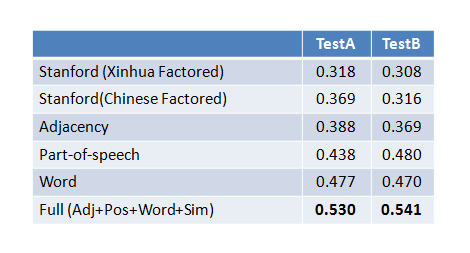
\includegraphics[scale=1]{uas.png}}
\caption{UAS results, comparing to an off-the-shelf Stanford Chinese dependency parser.}
\label{fig:uas}
\end{figure*}
\begin{figure*}[t]
\centerline{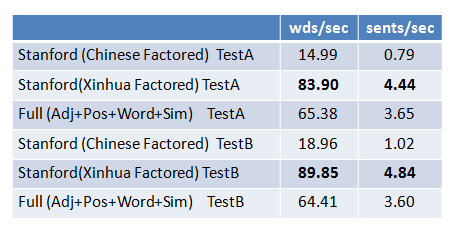
\includegraphics[scale=1]{speed.png}}
\caption{Runtime speed, comparing to an off-the-shelf Stanford Chinese dependency parser.}
\label{fig:speed}
\end{figure*}
Using the newly added similarity clauses, we obtain the final results in the Fig.~\ref{fig:uas}.
We see that the final performance is much better than an off-the-shelf Stanford Chinese
dependency parser. We also compare the runtime of our parser with the Stanford parser.
The results are shown in the Fig.~\ref{fig:speed}.
We see that although Stanford parser with the compact Xinhua model runs faster,
our model brings much better accuracy, without sacrificing much about the runtime.

\section{Conclusion and Future Work}
This work is among the first studies of dependency parsing for Weibo.
We also propose a novel dependency arc prediction approach based on an efficient probabilistic programming language.
Another contribution is that we provide the largest-ever FUDG-annotated GFL treebank (according to Lingpeng), for free.
Empirically, we obtain some interesting results on the Weibo data.
In the future, we plan to annotate more data, and explore more about joint intra-sentence and inter-sentence parsing.

\bibliographystyle{plainnat}
\bibliography{parsing}

\label{lastpage}
\end{document}
